\chapter{Contact Force-Torques and Internal Torques Estimation}
\label{chap:extForceAndJntTorqueEstimation}

\section{Introduction}
In this chapter we will discuss the techniques for whole-body external force-torque  and internal torques estimation developed to endow the iCub robot with torque-control capabilities. 
The developed techniques solved both the problems of \emph{external force-torque} and \emph{joint torques}, while the problem of identifying the \emph{location} of the external force-torque is solved using the distributed tactile system available on the iCub robot. 

This chapter extends the results presented in \citep{Fumagalli2012,DelPrete2016} and \citep{DelPrete2012} to the whole-body case. A key idea exploited in this chapter is that the rigid-body dynamics expressed w.r.t. to the \emph{proper sensor acceleration} is particularly well suited for force estimation, as the linear part of the  \emph{proper sensor acceleration} is exactly the output of an accelerometer mounted at the origin of the link. 

The chapter is structured as in the following. A brief state of the art of how this estimation problems have been solved in the past is presented in Section~\ref{sec:state-of-art-ft-estimation}. Section~\ref{sec:sensorModels} describe the different sensors used in the estimation algorithms. Section~\ref{sec:net-force-torque-estimation} discuss the estimation of the \emph{net force-torque} for a single rigid body. Section~\ref{sec:multibody-external-ft-estimation} introduces the algorithm for estimation of external force-torques of multibody system equipped with internal force-torques sensors. 
Section~\ref{sec:jointTorquesEstimation} discusses the estimation of joint torques, while Section~\ref{sec:model-based-ft-offset-calibration} discusses the estimation of six-axis force-torque sensor offsets. 

\section{State of art}
\label{sec:state-of-art-ft-estimation}

\subsection{Joint torques estimation}
Strain gauge-based direct sensing of joint torques is one of the main methods used to obtain joint torque feedback \citep{Wu1980, Luh1983}. Using this approach, the output shaft of the transmission of the motor system is modified to include a strain gauge, that is used to measure the deformation in the shaft due to the torque transmitted by the shaft to the system. The weak points of this techniques are the additional complexity added in the manufacturing of the motor group \citep{Randazzo2011} and the fact that strain-gauge sensor are quite sensitive to forces that exceed they sensing range. 

Another popular technique to estimate joint torque is the use of so-called Series Elastic Actuators (SEA) \citep{Paine2015}. In SEAs, a
linear compliant element (a ``spring'') is inserted in series after the transmission output shaft. Optical or magnetic encoders are mounted before and after the compliant element to measure its deformation, that is proportional to the transmitted torques. With respect to strain-gauge based techniques, there are two main advantages. The first one is to exploit explicitly designed compliance rather then the implicit compliance of the shaft, and the second one is to rely on optical or magnetic transducers, that are more robust then strain gauges. A drawback of SEAs is that while the additional compliance is convenient for torque measures, it may be a limitation for higher level controllers, not explicitly design to deal with a compliant system. For this reason the compliance level of a SEAs unit is tipically a tradeoff between the softness required for the torque measure and the rigidity required by classical high level controllers. 

An alternative to SEA-based torque estimation is to estimate the torque transmitted by the trasmission by measuring directly the deformation of the trasmission, rather then of a specifically designed elastic elements. In \citep{Zhang2015} in particular the authors use a pair of encoders to measure the deformation in a Harmonic Drive. With respect to classical SEA-based techniques, in the trasmission-based estimation the compliance model of the trasmission is not simply linear, but it is more complicated. 

All the discussed techniques until now (strain gauges mounted on the shaft, SEAs, trasmission-deformation) rely on specific hardware to measure the deformation of part of the motor group. Adding this specific hardware can be too costly, or simply unfeasible if a robot was already designed without any concern for torque control, as it was the case for iCub. An alternative is to estimate the joint torque from the motor input voltage or current, inverting a given model of relationship between the input variable of the motor and the output torques. This is feasible for low gear ratio motor groups as in \citep{WensingChetah2017}, but in classical robot system equipped with Harmonic Drives the effect of friction effects degrades the torque estimation quality. 

In this thesis we will present a technique for estimating the joint torques without any motor level sensor, but relying instead on six-axis force-torque sensor embedded in some of the robot links, as initially explored in \cite{Fumagalli2012}.

\subsection{External force-torque position estimation}
In general, external force-torques are exchanged over a surface at the interface between the robot and the environment, the so-called \emph{contact surface}. Estimating the contact surface is important mainly because it can be used by the robot to produce forces are prevent the contact to be broken. 

\citep{DelPrete2011} considered the problem of estimating the position of an external contact assuming that the contact generates a pure force (i.e. null torque) and its effects are sensed with a force/torque sensor embedded in the robot structure (e.g. at the robot base). The estimation relies on the classical force transformation principle \cite[Section 3.8.3]{Siciliano2009} according to which the spatial transformation of a pure force generates a torque equal to the cross product of the application vector and the applied force. Estimating the application vector (i.e. the contact location) boils down to a linear least squares which identifies a unique solution if at least two non collinear forces. The proposed procedure allows the calibration of a tactile array. In \citep{Manuelli2016} the authors propose to solve two problems simultaneously: contact location on the one hand and external force estimation on the other. To reduce the associated computational complexity, the two problems are separated to exploit the fact that the force estimation problem is convex if contact locations are known. The proposed estimation problem is solved with a particle filter. 

In this thesis, we will not presnt techniques for estimating the \emph{position} of an external force-torque, as we rely on  a distributed tactile system such as the one present in the iCub robot \cite{maiolino2013,DelPrete2011}.

\subsection{External force-torque intensity estimation}
\citep{DeLuca2006} proposed an approach to estimate the effect of external forces from joint torque measurements. Their approach is based on the definition of a dynamic quantity, the residual, which acts as a collision identification signal. Its has two main features: first, it can be computed from the motor torques and the joint positions and velocities; second, its dynamics are governed by a linear differential equation and therefore the residual is zero if no external contact force is applied to the manipulator. 
\citep{Magrini2014} proposed a contact estimation strategy which is based on the residual concept proposed by \citep{DeLuca2006}. The estimation of the contact location relies on a Kinect to detect the human posture and on a robot three dimensional rendering to predict possible contact location on the robot surfaces. Given the contact location, a least-square estimation is proposed to obtain the contact force magnitude and direction via a Moore-Penrose pseudo-inverse computation. Only the force components which do not lie on null space of the contact Jacobian can be estimated and this is a limitation of the proposed approach.
\citep{Park2005} considered the problem of estimating contact forces assuming a spring contact model for the external forces. A classical task-space inverse dynamics controllers is adopted to control contact forces. The proposed estimation technique, named Active Observer (AOB), consists of a Kalman filter for estimating the difference between the input command force and measured output force. \citep{Petrovskaya2007} extended the AOB estimator in \citep{Park2005} to include the geometric model of the interaction. In particular, the proposed approach defines a probabilistic model of the robot and the environment. The estimation strategy aims at estimating the position of the contact point on the robot, while maintaining constant the model of the environment. Estimation is limited to the single contact case even if experiments include some multi-contact scenarios handled with compliant exploration strategy described by \citep{Park2005}. 

In this thesis we present techniques for estimating the intensity of a group of external force-torque in the whole-body case relying on a distributed tactile system and on six-axis force-torque sensor embedded in some of the robot links, as initially explored in \citep{DelPrete2012}. As we assume that no joint torque measurement are available, we cannot use any residual-based technique.
 

\section{Sensor Models}
\label{sec:sensorModels}
In the previous chapter, we presented the theoretical background underling the dynamics of multibody systems.
In this section we will do a brief review of all the sensors that will be used in this and in the following chapters, and their relationship to the quantities that we defined in the previous chapters. For a detailed description of the underling physical principles, the interested reader is referred to \citep[Chapter 4]{doebelin2003}. 

\subsection{Joint Sensors}
\subsubsection{Six Axis Force Torque Sensor}
In the following, we will always model a six axis force torque sensor as a fixed joint,
that connects the two sides of the sensors.  This choice has the convenient condition that all the inertial information necessary to describe the sensor are still stored in the model description introduced in Chapter~\ref{chap:multibody}. Under this assumption, to fully describe a force-torque sensor we need the following information: the fixed joint of which the force-torque sensor measure the transmitted force-torque, the frame in which the force-torque sensors is reporting its measure, and the applied body on which the measured force-torque is assumed to be applied. For example, if two bodies $B$ and $D$ are rigidly attached by a fixed joint, and $\ls_B \rmf_{B,D}$ is the force-torque applied by $B$ on $D$, the measure force-torque is given by:
\begin{equation}
\label{eq:six-axis-ft-sensor}
y_{\text{FT}} = \sigma_{B,D} \ls_S X^B \ls_B \rmf_{B,D}
\end{equation}
where the constant $\sigma_{B,D} \in \{-1,1\}$ accounts for the \emph{direction} of the measured force-torque. 
\begin{remark}
In the next chapters, we will assume that joint-related quantities such as joint positions $s$, joint velocities $\dot{s}$ are measured. As the definition of these quantities is rather unambiguous given a multibody definition as in Chapter~\ref{chap:multibody}, we will not discuss their definition in detail. 
\end{remark}

\subsection{Link Sensors}
\label{subsec:linkSensors}
All the sensors in this subsection are assumed to be rigidly connected to a body, whose frame is indicated with $B$. Furthermore the sensors are assumed to be mounted such that they report their measurement in a frame $S$, rigidly attached to the body, while $A$ indicates as usual an inertial frame.

\subsubsection{3D Accelerometer} 
\label{subsec:accelerometer}
A 3D accelerometer is a sensor that measures the linear part of the \emph{proper sensor} acceleration of frame $S$, as described in Subsection~\ref{subsec:properAcceleration}:
\begin{equation}
y_{\text{acc}} = \ls^S R_A \ls^A \ddot{o}_S - \ls^S R_A \ls^A g
\end{equation}
Note that this definition is actually independent from the assumed inertial frame $A$.
\todo[inline]{Add reference to this as explained in wasref{inertialFrameInvariance}. }


\todo[inline]{In the following table we express this measurement w.r.t. the different representation of the body angular velocity: table velocity}

\subsubsection{3D Gyroscope} 
A 3D gyroscope is a sensor that measures the 3D angular velocity of the sensor frame $S$:

\begin{equation}
y_{\text{gyr}} = \ls^S \omega_{A,S} = ( \ls^A {R}_S^T  \ls^A \dot{R}_S )^\vee
\end{equation}
This measurement can identified simply as the angular part of the \emph{left-trivialized} velocity of the sensor frame $S$ w.r.t. to an inertial frame $A$:

\begin{equation}
y_{\text{gyr}} = \begin{bmatrix} 0_{3\times 3} & 1_3 \end{bmatrix}  \ls^S \rmv_{A,S} = \ls^S {\omega}_{A,S}.
\end{equation}

\subsubsection{3D Magnetometer}

The 3D magnetometer is a sensor that measures the magnetic field intensity in the sensor frame. In typical application scenario, it is assume that the measured magnetic field is the earth magnetic field $\ls^A b \in \mathbb{R}^3$, a quantity that can be assumed constant in the absolute frame $A$:
\begin{equation}
y_{\text{mag}} = \ls^S R_A \ls^A b = \ls^S R_B \ls^B R_A \ls^A b .
\end{equation}

\subsubsection{Inertial Measurement Unit}

An \emph{Inertial Measurement Unit} is a compound sensor in which a gyroscope, an accelerometer and possibly a magnetometer are packed together to estimate the orientation of the sensor frame w.r.t. an arbitrary \emph{earth-fixed} inertial frame $A_{\text{IMU}}$. The output of the IMU estimation is then an orientation, that can be expressed using Euler Angles, Quaternion or some other representation of $\SO(3)$. Assuming that we consider the output of the IMU to be directly a rotation matrix, we have:
\begin{equation}
y_{\text{IMU}} = \ls^{A_{\text{IMU}}} R_S = \ls^{A_{\text{IMU}}} R_A \ls^A R_B \ls^A R_S
\end{equation}
It is important to stress that in general the inertial frame $A_{\text{IMU}}$ used by the IMU may be different from the one used in the rest of the analysis. The constant $\ls^{A_{\text{IMU}}} R_A$ must be properly taken in account when designing algorithms that use the output of one or more IMUs.

\begin{remark}
The force-torque sensors, the gyroscope and accelerometer operating principle is actually always based on deformation or vibration: while this may seems a violation of the basic assumption of rigid body systems, the point is that the dynamics of such part of the systems is usually negligible w.r.t. the dynamics of the multibody system. 
For example, for a humanoid robot with a total mass of the order $10^2$ \si{Kg} where even smallest links have a mass in the order of $10^{-2}$ \si{Kg}, the proof mass of an accelerometers sensors can be in the order of $10^{-10}$ \si{Kg} \citep{andrejavsic2008mems}.
\end{remark}


\section{Estimation of the net force-torque}
\label{sec:net-force-torque-estimation}

\subsection{Example: rigid body external force-torque estimation}
Imagine that you have a rigid body $B$ attached to a bigger structure through a force-torque sensor and subject to an external force-torque due to the interaction with the environment, as depicted in Figure~\ref{fig:extFTsSingleBody}. Assuming for simplicity that the force-torque sensor returns the constraint force in the body frame $B$, we have from the rigid body dynamics of the body expressed w.r.t. \emph{proper sensor acceleration}:
\begin{equation}
\label{eq:Malphaetcetc}
    \ls_B \bbM_B\alpha^g_{A,B} + \begin{bmatrix} 
0_{3\times1} \\
\ls^B \omega_{A,B} 
\end{bmatrix}
\bar{\times}^*
\ls_B \bbM_B
\begin{bmatrix} 
0_{3\times1} \\
\ls^B \omega_{A,B} 
\end{bmatrix} = \ls_B \rmf^x +  \ls_B \rmf^s
\end{equation}

So, assuming a perfect model and the knowledge of the inertial parameters of the body, and measurements of $\alpha^g_{A,B}$, $\ls^B \omega_{A,B}$ and $\ls_B \rmf^s$ at a given instant, we can estimate the external force-torque $\ls_B \rmf^x$ as:
\begin{equation}
\label{eq:singleBodyForce}
    \ls_B \rmf^x = \ls_B \bbM_B \alpha^g_{A,B} + \begin{bmatrix} 
0_{3\times1} \\
\ls^B \omega_{A,B} 
\end{bmatrix}
\bar{\times}^*
\ls_B \bbM_B
\begin{bmatrix} 
0_{3\times1} \\
\ls^B \omega_{A,B} 
\end{bmatrix} -   \ls_B \rmf^s 
\end{equation}

Conveniently, in this formula the term $\bbM \alpha^g_{A,B} + \begin{bmatrix} 
0_{3\times1} \\
\ls^B \omega_{A,B} 
\end{bmatrix}
\bar{\times}^*
\ls_B \bbM_B
\begin{bmatrix} 
0_{3\times1} \\
\ls^B \omega_{A,B} 
\end{bmatrix}$ is the only one that depends  on acceleration, velocity and the inertial parameters of the body. For convenience, we will indicate this term as:
\begin{equation}
\ls_B \phi_B( \ls^B \alpha^g_{A,B}, \ls^B \omega_{A,B}) := \ls_B \bbM_B \alpha^g_{A,B} + \begin{bmatrix} 
0_{3\times1} \\
\omega_{A,B} 
\end{bmatrix}
\bar{\times}^*
\ls_B \bbM_B
\begin{bmatrix} 
0_{3\times1} \\
\ls^B \omega_{A,B} 
\end{bmatrix}
\end{equation}

In the following we will omit the dependency on the \emph{proper sensor acceleration} and on the \emph{body angular velocity} and simply indicate this as $\ls_B \phi_B$. An interpretation for the physical meaning of $\ls_B \phi_B$ is that is the sum of all the force-torque acting on body, both the external ones and the one due to interaction with the other bodies in the system, minus the gravitational force-torque. Even if this term does not include the force-torque due to gravity, to simplify the nomenclature in the following will call it \emph{net force-torque} acting on the body $B$.

Using the definition of net force-torque, the external force-torque estimation can be compactly expressed as:
\begin{equation}
\label{eq:extforce-torque}
    \ls_B \rmf^x = \ls_B \netFT_B -   \ls_B \rmf^s 
\end{equation}

\begin{figure}
\begin{tikzpicture}
\node[inner sep=0pt] (floatingBase) at (0,0) {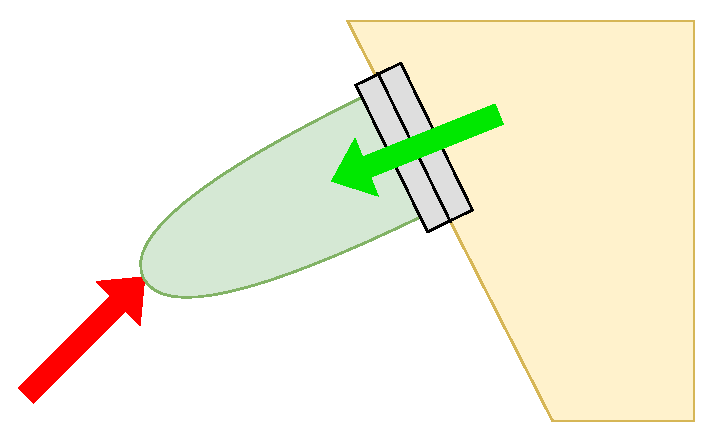
\includegraphics[width=\linewidth]{Figs/thesis-single-body-wrench.eps}};
\node[inner sep=0pt] (B) at (-1.0,1.0) {\Huge $B$};
\node[inner sep=0pt] (extFT) at (-4.0,-2.0) {\Huge ${\ls_B \rmf^x}$};
\node[inner sep=0pt] (measFT) at (3.0,2.0) {\Huge ${\ls_B \rmf^s}$};
\end{tikzpicture}
\caption{Graphical rappresentation of equation \eqref{eq:extforce-torque}.}
\label{fig:extFTsSingleBody}
\end{figure}

The net force-torque $\ls_B \netFT^B$ of body $B$ depends on the inertial parameters of the body $B$, the \emph{proper sensor acceleration} and on the \emph{body angular velocity}. In this chapter, we assume that the inertial parameters of the body are perfectly known. Techniques to estimate those parameters are discussed in Chapter~\ref{ch:inertialParameters} and Chapter~\ref{ch:inertialParametersMultiBody}. 

If these inertial parameters are assumed to known, then the \emph{net force-torque} estimation boils down to estimation of the \emph{proper sensor acceleration} $\alpha_{A,B}^g$ and on the \emph{body angular velocity} $\ls^B \omega_{A,B}$.

\subsection{Sensor based estimation}
Beside the inertial parameters, to compute the net force-torque it is necessary to estimate the proper sensor acceleration $\alpha^g_{A,B} \in \R^6$ and the \emph{body} angular velocity $\ls^B \omega_{A,B} \in \R^3$. In an ideal case, we would want to have a linear accelerometer, and angular accelerometer and a gyroscope rigidly mounted on the body, all reporting their measurements directly in the body frame $B$. 
However, typically this is not the case. Firstly there could be an offset between the sensor frame $S$ and the body frame $B$. Secondly, angular accelerometers are not tipically available as off-the-shelf component, and so the information on the angular acceleration is typically obtained by numerical derivative of the gyroscope output. Another strategy used to deal with the absence of direct angular acceleration feedback is to simply ignore the angular acceleration contribution to the net force-torque, assuming its influence in the overall dynamics to be negligible.

Assuming that one of the above strategies was used to compute $\ls^S \dot{\omega}_{A,S}$, we will have a \emph{proper sensor acceleration} $\alpha_{A,S}^g$ and an angular velocity expressed $\ls^S \omega_{A,S}$, and we want to transform them in the frame $B$, in which the rest of the model information (such as inertial parameters and joint information) is expressed. From the definition of sensor acceleration and from the propagation rules for mixed acceleration \eqref{eq:accelerationPropagationMixed} we have that:
\todo[inline]{Simplify this expression to highlight the dependency on sensor measurements}
\begin{IEEEeqnarray}{rCl}
\label{eq:accFromIMUtoLink} \IEEEyesnumber
    \ls^B \omega_{A,B} &=& \ls^B R_S \ls^S \omega_{A,B}, \IEEEyessubnumber \\
    \alpha_{A,B}^g &=& \ls^B X_S  \alpha_{A,S}^g + 
    \begin{bmatrix} 
    \ls^B \omega_{A,B}^\wedge \ls^B \omega_{A,B}^\wedge \ls^B o_S \\
    0_{3 \times 1}
    \end{bmatrix}.  \IEEEyessubnumber
\end{IEEEeqnarray}


\subsection{Kinematic based estimation}
\label{subsec:kinematicBaseEstimation}
In humanoid robotics, it is actually unusual to have more then one IMU mounted on the robot. Typically only one IMU is mounted on one \emph{central} link of the robot, and information on the angular velocity and proper sensor acceleration of all the other links can be obtained through kinematic propagation, using information about joint velocity $\dot{s}$ and acceleration $\ddot{s}$. This information can be obtained thought high-frequency numerical derivation of high-precision joint encoders.

Under this assumption, we can compute recursively the angular velocity and proper sensor acceleration, considering the \emph{base link} $B$ to be the one in which the IMU is available. In particular we assume that we can compute $\alpha^g_{A,B}$ and $\ls^B \omega_{A,B}$ for the link containing the IMU using equations \eqref{eq:accFromIMUtoLink}. Then, given an arbitrary link $L$, its sensor proper acceleration and body angular velocity can be computed from \eqref{eq:accelerationPropagationSensor} and \eqref{eq:velocityPropagationLeft}:
\begin{IEEEeqnarray}{rCl}
\IEEEyesnumber 
\ls^L \omega_{A,L} &=& \ls^L R_B(s) \ls^B \omega_{A,B} + \ls^L \omega_{B,L}(s,\dot{s}),
\IEEEnonumber \\
\alpha_{A,L}^g &=& \ls^{L} X_{B}(s) \alpha_{A,B}^g + \alpha_{B,L}(s,\dot{s},\ddot{s}) + \\ 
        && \begin{bmatrix}
          \ls^L R_B(s) \left[ 2 ( \ls^B \omega_{A,B} \times \ls^B \dot{o}_L(s,\dot{s}) ) +  \ls^B \omega_{A,B} \times (\ls^B \omega_{A,B} \times \ls^B o_L(s) ) \right] \\
         \left( \ls^L R_B(s) \ls^B \omega_{A,B} \right)^\wedge \ls^L \omega_{B,L}(s,\dot{s})
          \end{bmatrix} = \\
          &=& \ls^{L} X_{B}(s) \alpha_{A,B}^g + \alpha_{B,L}(s,\dot{s},\ddot{s}) + \\
          &&
          \begin{bmatrix} 2 \ls^L R_B(s) \ls^B \omega_{A,B}^\wedge & 0_{3 \times 3} \\ 
                          0_{3 \times 3} & \ls^L R_B(s) \ls^B \omega_{A,B}^\wedge
          \end{bmatrix} \ls^{L[B]} \rmv_{L,B} + \\
          && 
          \begin{bmatrix}
          \ls^L R_B(s) [ \ls^B \omega_{A,B} \times (\ls^B \omega_{A,B} \times \ls^B o_L(s) ) ] \\
          0_{3 \times 1}
          \end{bmatrix}
\IEEEnonumber 
\end{IEEEeqnarray}
where $\ls^L R_B(s), \ls^{L} X_{B}(s), \ls^L \omega_{B,L}(s,\dot{s})$, $\ls^B \dot{o}_L(s,\dot(s))$ and $\alpha_{B,L}(s,\dot{s},\ddot{s})$ are given by the relative forward kinematics.



\begin{comment} 
% ADD it back if we put the chapter on algorithms
% This is actually  important because it is how we actually we perform this computation. 
In theory, one can compute the joint propagation for the $\emph{proper sensor}$ acceleration equation. However, this is an equation with four terms, that can be difficult to properly code in software. Furthermore, as explained in \ref{} the kinematic propagation are typically implemented in software using the \emph{left-trivialized} velocity representation. Consequently, we can use this representation also in this case, by noting that yetToBeNamed can be also be expressed as 
$$
\ls_L \phi_L = L_L \mathbb{M}_L \ls^L \rma^g_{A,L} + \ls^L \rmv_{A,L} \bar{\times}^* L_L \mathbb{M}_L \ls^L \rmv_{A,L}
$$
We can then compute $\ls_L \phi_L$ by using the left-trivialized velocity of each link, that we can compute using the kinematic loop of the RNEA, using the link equipped with an IMU as the base link. The only difference in this case is that the left-trivialized proper base acceleration and the left-trivialized velocity are computed from the proper sensor acceleration and the angular velocity. While for performing this computation we actually need a value for the linear part of the left-trivialized velocity, the actual values of the net force-torque is indipendent from its value, an so we can choose any arbitrary value. Pay attention that anyhow the linear part of the computed velocities will not be identically zero, because they will contain the linear velocity due to the angular velocity of the joints.. However this linear velocity will not have any physical meaning. 
\end{comment}

% This is similar to the 

\subsection{Hybrid estimation}
It only a $n_{IMU}$ out of $\nLinks$ links of the of the robot are equipped with IMUs, it is possible to mix the two approaches by splitting the multibody system in $n_{IMU}$ submodels, each of it containing several connected links, of which only one is equipped with an $IMU$. For all other links in the subgraph, the net force-torque of each link can be computed by propagating the the kinematic information using the joint information, using the equations presented in the previous subsection. 


\section{Multibody External Force-Torque Estimation}
\label{sec:multibody-external-ft-estimation}
\subsection{Force-Torque Sensors Induced Submodel Decomposition}
\label{subsec:modelDecomposition}
In this section we consider the generalization of single-body external force-torque estimation depicted in Fig~\ref{fig:extFTsSingleBody} to the multibody case, depicted in Figure~\ref{fig:extFTsMultiBody}.

For exploiting the measures of internal force-torque sensors, it is convenient to consider independently each submodel induced by cutting the multibody-model along the fixed joints that contain an internal force-torque sensor. If we have $n$ force-torque sensors, we can define $n+1$ submodels. We indicate with $\mathfrak{M}$ the set of different submodels, with $sm \in \mathfrak{M}$ a specific submodel, and with $\linkSet_{sm}$ the set of the links belonging to submodel $sm$. 

Furthermore, for each link $L \in \linkSet_{sm}$ we indicate with $\beth_{sm}(L)$ the set of links that are connected with $L$ in the full model, but that belong to a different submodel, i.e.: 
\begin{equation}
\beth_{sm}{(L)} := \{ D \in \linkSet \  | \  \{L,D\} \in \jointSet \land D \notin  \linkSet_{sm}\} 
\end{equation}


\begin{figure}
\begin{tikzpicture}
\node[inner sep=0pt] (floatingBase) at (0,0) {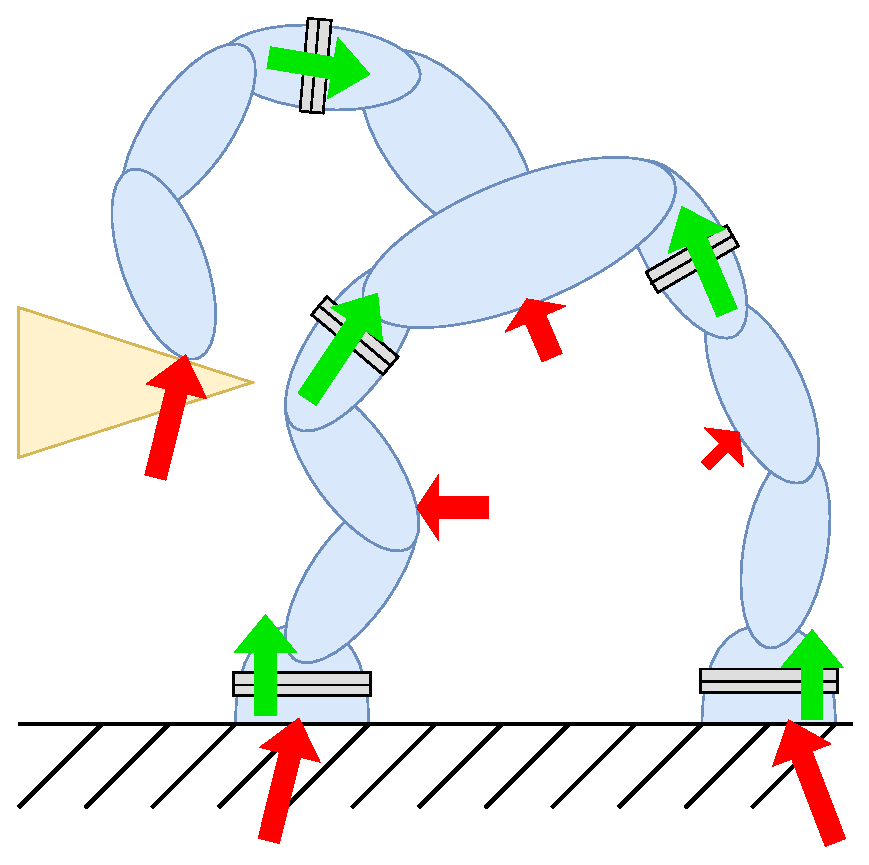
\includegraphics[width=\linewidth]{Figs/thesis-submodel-decomposition.eps}};
% \node[inner sep=0pt] (B) at (-1.0,1.0) {\Huge $B$};
% \node[inner sep=0pt] (extFT) at (-4.0,-2.0) {\Huge ${\ls_B \rmf^x}$};
% \node[inner sep=0pt] (measFT) at (3.0,2.0) {\Huge ${\ls_B \rmf^s}$};
\end{tikzpicture}
\caption{Example of a multibody system with internal six-axis force-torque sensors. Measured force-torques are indicated in green, while unknown contact force-torques are drawn in red. There are $n = 5$ force-torque sensor in the system, that is then decomposed in $n+1 = 6$ submodels for external force-torque estimation.}
\label{fig:extFTsMultiBody}
\end{figure}


\subsection{External Force-Torque Estimation}
In the following, we will use this assumptions. 

\begin{assumption}
The contact surface and the link to which it belongs of the  external force-torques are both known, either from a-priori assumptions or from the measurements from a distributed tactile skin. The a-priori assumptions or the skin do not provide information on the \emph{intensity} of the external force-torque. 
\end{assumption}

\begin{assumption}
The net force-torque $\ls_L \netFT_L$ of each link is assumed to be known, estimated using one of the techniques described in Section~\ref{sec:net-force-torque-estimation}. 
\end{assumption}


\begin{property}
\label{prop:ne-for-link-in-multibody}
Given a link $L \in \linkSet$ the relation between the net force-torque $\ls_L \phi_L$,  the net external force-torque $\ls_L \rmf^x_B$ and the joint internal force-torques is given by:
\begin{equation}
\label{eq:ne-for-link-in-multibody}
   \ls_L \phi_L = \ls_L \rmf^x_L + \sum_{D \in \aleph(L)} \ls_L \rmf_{D,L}.
\end{equation}
\end{property}
This equation is just a generalization of \eqref{eq:Malphaetcetc} to all the forces interacting with a given link in a multibody system. 

A similar result holds for the multibody system as an whole, as stated in the next Proposition. 
\begin{theorem} 
\label{thm:full-body-newton-euler}
Given a multibody system in which the external force-torques are acting on only a subset of the links $\mathfrak{C} \subseteq \linkSet$, the sum of all the net force-torques of each link is equal to the sum of all the external force-torques acting on the multibody system, provided that all quantities are transformed in a common frame $B$, i.e. :
\begin{equation}
    \label{eq:NEforEstimationCompleteModel}
    \sum_{L \in \mathfrak{L}}  \ls_B X^L \ls_L \phi_L = \sum_{L \in \mathfrak{C}} \ls_B X^L \ls_L \rmf^x_L .
\end{equation}
\end{theorem}
The proof of this theorem is given in Subsection~\ref{proof:full-body-newton-euler}.

With respect to the single body case using Theorem~\ref{thm:full-body-newton-euler} we can only estimate the sum of all the external force-torque acting on the multibody system. However it is typically of interest to estimate the intensity of each contact force-torque independently from the others, for example for force control. On the other hand, we need to use in some way the information coming from the force-torque sensor, that measure \emph{internal} force-torque, to estimate \emph{external} force-torque. 

A way of obtaining an equation similar to Theorem~\ref{thm:full-body-newton-euler}  that contains the available sensors measures, is to split the multibody model in several submodels, along the joints in which force-torque sensors are mounted, as described in Subsection~\ref{subsec:modelDecomposition}. We can then apply Theorem~\ref{thm:full-body-newton-euler} to each submodel $sm \in \mathfrak{M}$, that we can rewrite as:
\begin{equation}
    \label{eq:NEforEstimationSubModel}
    \sum_{L \in \linkSet_{sm}}  \ls_B X^L \ls_L \phi_L = \sum_{L \in (\mathfrak{C} \cap \linkSet_{sm}) }  \ls_B X^L \ls_L \rmf^x_L +  \sum_{L \in \mathfrak{L}_{sm}} \sum_{D \in \beth_{sm}(L)}  \ls_B X^D \ls_D \rmf_{D,L} .
\end{equation}

The term $\sum_{L \in \mathfrak{L}_{sm}} \sum_{D \in \beth_{sm}(L)}  \ls_B X^D \ls_D \rmf_{D,L}$ represents the effect on the submodel of the force-torques transmitted by the six-axis sensors. For a given force-torque sensor embedded in the joint $\{D,L\} \in \jointSet$, the value of $\ls_D \rmf_{D,L}$ can obtained from the sensor measurement $y_{FT}$ by inverting equation~\eqref{eq:six-axis-ft-sensor}:
\begin{equation}
\label{eq:inverse-ft-sensor-equation}
\ls_D \rmf_{D,L} = \ls_D X^S \sigma_{D,L} y_{\text{FT}}.
\end{equation}

In the rest of the chapter we will assume that the joint force-torque $\ls_D \rmf_{\{D,L\}}$ is always available for each joint in which a six-axis force-torque sensors is mounted, without manually indicating its value from equation \eqref{eq:inverse-ft-sensor-equation}.

Given a submodel $sm \in \mathfrak{M}$, if we assume that on the submodel the external force-torques are acting only on a single link called $C$ (i.e. $(\mathfrak{C}~\cap~\linkSet_{sm}) = \{C\}$) then this external force-torque can be computed exactly from \eqref{eq:NEforEstimationSubModel} as:
\begin{equation}
   \ls_{C} \rmf^x_{C} =
   \sum_{L \in \linkSet_{sm}}  \ls_C X^L \ls_L \phi_L   -  \sum_{L \in \mathfrak{L}_{sm}} \sum_{D \in \beth_{sm}(L)}  \ls_C X^D \ls_D \rmf_{D,L} .
\end{equation}

\subsection{Estimation of external forces acting on multiple link in a submodel}
If the external forces are acting on more then one link, the estimation problem given by \eqref{eq:NEforEstimationSubModel} is indeterminate, as the number of unknowns is greater then 6, the number of given equations. A possible solution in this case is to solve the equation in the least-square sense as proposed in \cite{DelPrete2012}, but in this case there is no guarantee that the resulting estimated force-torques are the ``real'' ones. In this sense, the least-square estimation should be seen as fallback solution, rather then a sound estimation technique. 

\section{Joint Torques Estimation}
\label{sec:jointTorquesEstimation}
Once we obtained a set of external force-torques, a strictly related problem is how to estimate the internal torques, i.e. the component of the inter-link forces acting along the degree of freedom of the joints. The joint torques estimation is crucial because this quantity is directly related to the motors that are actuating those joints, and the input to the motors is in the end the ultimate control input available in robots. 

We have that the torques of the joint connecting links $E$ and $F$ are just the projection of the joint force-torque on the joint motion subspace:
\begin{equation}
\label{eq:jointTorqueFromInternalSimple}
\tau_{\{E,F\}} = \left< \ls^F \mathrm{s}_{E,F}, \ls_F \rmf_{E,F} \right> = \left< \ls^E \mathrm{s}_{F,E}, \ls_E \rmf_{F,E} \right> .
\end{equation}
The joint torque estimation problem is then solved if an estimation of the joint internal force-torque is available. The internal force-torque estimation problem has a trivial solution using the following property.

\begin{definition}
\label{def:consistent-force-torques}
A set of estimated net force-torques $\ls_L \phi_L, \ L \in \linkSet$ and of external force-torques $\ls_L \rmf^x_L, \ L \in \linkSet$ is \emph{consistent} if they follow equation \eqref{eq:NEforEstimationCompleteModel}.
\end{definition}

\begin{property}
\label{prop:ext-forces-estimation-is-consistent}
The outcome of the estimation of force-torques algorithm presented in Section~\ref{sec:multibody-external-ft-estimation} is always consistent, as defined in Definition~\ref{def:consistent-force-torques}.
\end{property}

Given a set of net force-torques for each body and a set of \emph{consistent} external force-torques, all the internal joint force-torques are totally determined. In particular, the internal force-torque can be written in two equivalent ways: 
\begin{IEEEeqnarray}{rCl}
\label{eq:internalforce-torqueFromNetAndExternal}
\IEEEyesnumber 
 \ls_F \rmf_{E,F}  &=& - \ls_E \rmf_{F,E}\IEEEyessubnumber \\ 
\ls_F \rmf_{E,F} &=& \sum_{L \in \gamma_E(F)} \ls_F X^L  \left( \ls_L\phi_L + \ls_L\rmf^x_L \right) \IEEEyessubnumber \label{eq:otherExpressionForInternalFT} \\
\ls_E \rmf_{F,E} &=& \sum_{L \in \gamma_F(E)} \ls_E X^L \left( \ls_L\phi_L + \ls_L \rmf^x_L  \right) \IEEEyessubnumber \label{eq:oneExpressionForInternalFT} 
\end{IEEEeqnarray}
where $\gamma_E(F)$ is the set of the links belonging to the subtree starting at link $F$, given $E$ as a base link, defined originally in Definition~\ref{def:subtreeLinks}. 

The two sums are equivalent thanks to the fact the the net force-torques and the external force-torques are \emph{consistent}. 

Combining equations \eqref{eq:internalforce-torqueFromNetAndExternal} and \eqref{eq:jointTorqueFromInternalSimple} is is possible to estimate the joint torques using net force-torques as estimated in Section~\ref{sec:net-force-torque-estimation} and external force-torques estimated in Section~\ref{sec:multibody-external-ft-estimation} :
\begin{IEEEeqnarray}{rCl}
\IEEEyesnumber
\label{eq:jointTorqueFromNetAndExternal}
\tau_{ \{E,F\}} 
&=& \left< \ls^F \mathrm{s}_{E,F}, \sum_{L \in \gamma_E(F)} \ls_F X^L  \left( \ls_L\phi_L + \ls_L\rmf^x_L \right) \right> = \IEEEyessubnumber \\
&=& \left< \ls^E \mathrm{s}_{F,E}, \sum_{L \in \gamma_F(E)} \ls_E X^L \left( \ls_L \phi_L + \ls_L\rmf^x_L  \right) \right> \IEEEyessubnumber .
\end{IEEEeqnarray}


Note that \eqref{eq:jointTorqueFromNetAndExternal} is just an alternative formulation for the line of \eqref{eq:multibodyEqsOfMotWithSensorAcc} relative to $\tau_{\{E,F\}}$, and it is usually computed using the algorithms for computing \emph{Inverse Dynamics} \citep{featherstone2008}.

Relying on \eqref{eq:jointTorqueFromNetAndExternal} for internal force-torque estimation may seem risky, as it create a dependency of the torques on the net force-torque and external force-torque of the link of all the robot, and this could be be subject to accumulation error. In the next theorem we see how most of the torques computed as in \eqref{eq:jointTorqueFromNetAndExternal} are actually function of a much more ``local set of measurements''.

\begin{theorem}
\label{thm:torqueEstimationIsLocal}
Assume that:
\begin{itemize}
\item $(E,F)$ is a 1-dof joint, 
\item $(G,H)$ is a fixed joint that contains a force-torque sensor,
\item $F$ is closer to $G$ then $E$ (i.e. $G \in \gamma_E(F)$).
\item the path connecting $(E,F)$ to $(G,H)$ is branchless,
\item the path connecting $(E,F)$ to $(G,H)$ is free of external force-torques and other force-torque sensors,
\item $E$, $F$ and $G$ belong to the submodel $sm \in \mathfrak{M}$.
\end{itemize}
Then $\tau_{ \{ E,F \} }$ given by \eqref{eq:jointTorqueFromNetAndExternal} can be equivalently written as:
\begin{equation}
\label{eq:localTorqueEstimation}
\tau_{\{E,F\}} = \left< \ls^F \mathrm{s}_{E,F} , \sum_{ \gamma_E(F) \cap \mathfrak{L}_{sm}} \ls_F X^L  \ls_L \phi_L + \ls_F X^G \ls_G \rmf_{G,H} \right> .
\end{equation}
\end{theorem}

\begin{remark}
This means that the torque estimate is just a linear function of the force-torque sensor measure and of the net force-torque of a a limited set of links, the one connecting the joint $\{ E,F \}$ to the joint $\{ G, H \}$. This ensure that any error in all the other force-torque sensors measurements or in the estimation of net force-torque of all the other links in the robot will not influence the estimation of $\tau_{\{E,F\}}$. 
\end{remark}

\subsection{Example of torque estimation}
Let's focus on the upper part of the model depicted in Figure~\ref{fig:extFTsMultiBody}, depicted in \ref{fig:local-torque-estimation}. 

\begin{figure}
\centering
\begin{tikzpicture}
\node[inner sep=0pt] (floatingBase) at (0,0) {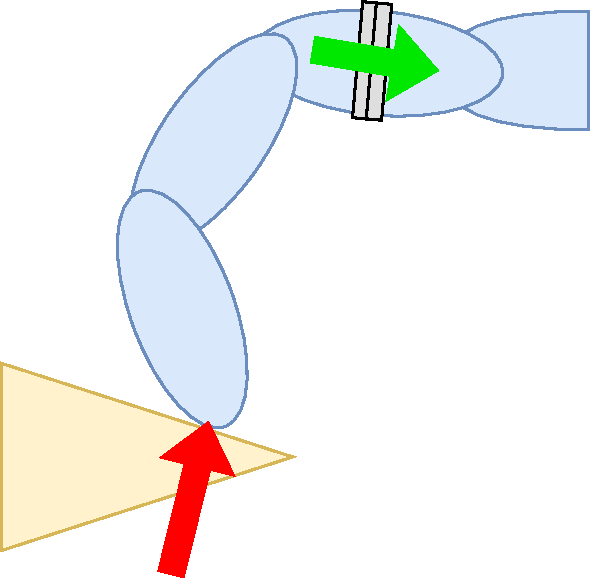
\includegraphics[width=0.6\linewidth]{Figs/local-torque-estimation.eps}};
\node[inner sep=0pt] (E) at (-1.6,-0.5) {\Huge $E$};
\node[inner sep=0pt] (F) at (-1.0,2.0) {\Huge $F$};
\node[inner sep=0pt] (G) at (0.5,3.5) {\Huge $G$};
\node[inner sep=0pt] (H) at (2.0,3.0) {\Huge $H$};
\end{tikzpicture}
\caption{Example of torque estimation.}
\label{fig:local-torque-estimation}
\end{figure}


As explained in this section, the joint torques can simply be estimated by \eqref{eq:jointTorqueFromNetAndExternal}, i.e. \emph{inverse dynamics}, once a \emph{consistent} set of net force-torques and external force-torques have been estimated. 
However, it is interesting to see on which measurements the estimate of the joint $\{ E, F\}$ actually depends on, using Theorem~\ref{thm:torqueEstimationIsLocal}. 
In this case we have that $\linkSet_{sm} = \{ D, E, F, G \}$ and $\gamma_E(F) \cap \linkSet_{sm} = \{ F, G \}$. Writing \eqref{eq:localTorqueEstimation} in this specific case we have:
\begin{equation}
\label{eq:localTorqueEstimationExample}
\tau_{\{E,F\}} = \left< \ls^F \mathrm{s}_{E,F} , \ls_F \phi_F +
\ls_F X^G \ls_G \phi_G + \ls_F X^G \ls_G \rmf_{G,H} \right> ,
\end{equation}
where $\ls_G \rmf_{G,H}$ is obtained directly from the force-torque sensor measurements. 
In the end the estimates of the joint $\tau_{\{E,F\}}$ depends only on the net force-torque of links $F$ and $G$ ($\ls_F \phi_F , \ls_G \phi_G$), on the measurement of the position of joint $\{ F, G \}$ and its geometrical model ($\ls_F X^G$) and on the measurement of the nearby force-torque sensor mounted on joint $\{G,H\}$ ($\ls_G \rmf_{G,H}$). Then, all other estimation errors that could be present on the robot do not affect the estimate of $\tau_{\{E,F\}}$, even if they are present in equation \eqref{eq:jointTorqueFromNetAndExternal}. 


\section{Six-Axis Force-Torque Sensors Model-based Offset Calibration} 
\label{sec:model-based-ft-offset-calibration}
As will be described in detail in \ref{chap:ft-calib}, the six-axis force-torque sensors bias needs to be determined during the startup of the system. For this reason, we need to have a way find the expected value of the measured sensor assuming the perfect knowledge of the model and some additional assumptions on the external force-torque. 

\subsection{Offset Calibration with the external forces acting on a Single Link}
\begin{assumption}
\label{ass:ft-calibration-on-single-link}
During force-torque bias sensor calibration, we assume that only one external force-torque is acting on the multibody system. We call $C$ the link on which the unique external 6D force is acting.
\end{assumption}

\begin{remark}
Assumption~\ref{ass:ft-calibration-on-single-link} can be automatically checked using a distributed tactile system. 
\end{remark}

If only one external force-torque is acting on the system, its value can be computed from Newton-Euler equations, using Theorem~\ref{thm:full-body-newton-euler}:
\begin{equation}
\label{eq:ft-external-force-torque-single-body}
\rmf^x_C = \sum_{L \in \mathfrak{L}}  \ls_B X^L \ls_L \phi_L
\end{equation}

Once the unique external force-torque has been determined using, joint force-torque for each joint can be computed using the equations in \eqref{eq:internalforce-torqueFromNetAndExternal}. In particular only one of the two equations \eqref{eq:oneExpressionForInternalFT}-\eqref{eq:otherExpressionForInternalFT} will contain the term related to external force-torque. By choosing the other expression for all the joints, the joint force-torque can be written as a function of the net force-torques. In particular given a joint $\{ E,F \}$, using $C$ as the base assume that $\lambda_C(F) = E$. Then $\gamma_E(F) = \gamma_C(F)$ and:
\begin{equation}
\ls_F \rmf_{E,F} = \sum_{L \in \gamma_C(E)} \ls_F X^L \phi_L .
\end{equation}

% \subsection{Offset Calibration with External Forces acting on Two Links}
% \label{subsec:macumba}

% In some real world scenarios, assumption~\ref{ass:ft-calibration-on-single-link} can be too restricting. If for example a humanoid robot is started directly standing on its two feet, the assumption is not respected until a foot is lifted. To deal with this case, we also defined a offset calibration procedure with a less restrictive assumption. 
% \begin{assumption}
% \label{ass:ft-calibration-on-two-links}
% If an offset estimation is performed when the external forces are acting on two links of the robot, we assume that 
% \end{assumption}


\todo[inline]{Example of iCub links} 

\section{Proofs}
\subsection{Proof of Theorem~\ref{thm:full-body-newton-euler}}
\label{proof:full-body-newton-euler}
We can sum the equations given by \eqref{eq:ne-for-link-in-multibody} for each link $L$ by multiplyng them for $\ls_B X^L$, resulting in:
\begin{IEEEeqnarray}{rCl}
\sum_{L \in \linkSet} \ls_B X^L \ls_L \phi_L &=& \sum_{L \in \linkSet} \ls_B X^L \left( \ls_L \rmf^x_L + \sum_{D \in \aleph(L)} \ls_L \rmf_{D,L} \right) = \IEEEnonumber \\
&=& \sum_{L \in \linkSet} \ls_B X^L \ls_L \rmf^x_L +  \sum_{L \in \linkSet} \sum_{D \in \aleph(L)} \ls_B \rmf_{D,L} . 
\label{eq:sum-of-ne-for-each-link}
\end{IEEEeqnarray}

Focusing on the last addend of the right term of the equation we have:
\begin{IEEEeqnarray}{rCl}
\sum_{L \in \linkSet} \sum_{D \in \aleph(L)} \ls_B\rmf_{D,L} &=& \IEEEnonumber \\
= \sum_{\{ E,F\} \in \jointSet} \ls_B\rmf_{E,F} + \ls_B\rmf_{F,E} &=& \IEEEnonumber  \\
=
\sum_{\{ E,F\} \in \jointSet} \ls_B\rmf_{E,F} - \ls_B\rmf_{E,F} &=& 0_{6 \times 1}
\label{eq:internal-forces-sum-to-zero}
\end{IEEEeqnarray}

Plugging \eqref{eq:internal-forces-sum-to-zero} in \eqref{eq:sum-of-ne-for-each-link} one obtains \eqref{eq:NEforEstimationCompleteModel}.

$\hfill\blacksquare$

\subsection{Proof of Theorem~\ref{thm:torqueEstimationIsLocal}}
From \eqref{eq:jointTorqueFromNetAndExternal} we have:
\begin{equation*}
\tau_{\{E,F\}} = \left< \ls^F \mathrm{s}_{E,F}, \ls_F \rmf_{E,F} \right> =  \left< \ls^F \mathrm{s}_{E,F}, \sum_{L \in \gamma_E(F)} \ls_F X^L  \left( \ls_L\phi_L + \ls_L\rmf^x_L \right) \right>
\end{equation*}

From \eqref{eq:otherExpressionForInternalFT} instead we have that:
\begin{equation}
\label{eq:sensor-force}
\ls^G \rmf_{G,H} = \sum_{L \in \gamma_G(H)} \ls_G X^L  \left( \ls_L\phi_L + \ls_L\rmf^x_L \right),
\end{equation}

and that:
$$
\gamma_E(F) = \left( \gamma_E(F) \cap \linkSet_{sm} \right) \cup \gamma_G(H).
$$

We can then decompose the expression of $\ls^F \rmf_{E,F}$ as:
\begin{IEEEeqnarray*}{rCl}
\ls^F \rmf_{E,F} &=& 
\sum_{L \in \gamma_E(F)} \ls_F X^L  \left( \ls_L\phi_L + \ls_L\rmf^x_L \right) = \\
&=& 
\sum_{L \in \gamma_E(F) \cap \linkSet_{sm} } \ls_F X^L  \left( \ls_L\phi_L + \ls_L\rmf^x_L \right) +
\sum_{L \in \gamma_G(H)  } \left( \ls_F X^L   \ls_L\phi_L + \ls_L\rmf^x_L \right) = \\
&=& 
\sum_{L \in \gamma_E(F) \cap \linkSet_{sm} } \ls_F X^L \left(  \ls_L\phi_L \right) + \ls_F X^G \ls_G \rmf_{G,H},
\end{IEEEeqnarray*}
where we made use of the assumption that no external force-torques are present on the links in $\gamma_E(F) \cap \linkSet_{sm}$ and the expression of $\ls_G \rmf_{G,H}$  given in \eqref{eq:sensor-force}.
Substituting this expression of $\ls_F \rmf_{E,F}$ in \eqref{eq:jointTorqueFromNetAndExternal} gives the result. 
$\hfill\blacksquare$